% Provenance (never printed): see sources/outline_sources.md (Year 3: the main
% field and its secular variation, rock magnetism, palaeomagnetic poles, apparent
% polar wander, magnetostratigraphy, the geodynamo). Brief: sources/book5/BRIEFS.md,
% ch. 4. Curves and maps from figdata/bachelor-3/igrf_field.py (IGRF-14),
% palaeomag_stats.py (the invented Kesta terrane, its Fisher statistics, the
% Zijderveld specimen and the reference APW path), magnetostratigraphy.py.
% Exercise and problem values in the Book 5 scratch calculator calc/ch04.py.
\chapter{भू-चुंबकत्व और पुराचुंबकत्व}\label{ch:b3:palaeomagnetism}

साठ मिलियन वर्ष पहले उद्गारित एक बेसाल्ट प्रवाह ठंडा होते समय अपने मैग्नेटाइट के सूक्ष्म कणों को
तत्कालीन क्षेत्र के समानांतर स्थिर कर चुका था; आज इसे ड्रिल करके, स्थान पर ही अभिविन्यस्त करके,
छोटे बेलनों में काटकर और वर्तमान क्षेत्र से परिरक्षित कक्ष में चरणबद्ध ढंग से गरम करके भी
वह चट्टान बताती है कि वह तब ध्रुव से कितनी दूर थी
और किस दिशा में उन्मुख थी।
हज़ारों ऐसे मापनों ने, हर महाद्वीप और हर युग से, यह बताया है कि
महाद्वीप उन महासागरीय तलों के जन्म से पहले कैसे खिसके, जो उनकी गति को अभिलिखित करते हैं,
और अवसादी अनुक्रम की परतों से होकर क्षेत्र किस क्रम में उत्क्रमित हुआ।
यह अध्याय आज के क्षेत्र का वर्णन करता है, चट्टानें उसे कैसे अभिलिखित करती हैं,
एक दिशा कैसे निकाली और औसत की जाती है,
और एक पुराचुंबकीय ध्रुव प्लेट की गति के बारे में क्या कहता है।

\begin{recall}
पृथ्वी का एक चुंबक के रूप में होना और चुंबकीय क्रांति भौतिकी की पुस्तकों के
विद्यालय-स्तरीय खंडों में हैं; चुंबकीय डोमेन, हिस्टैरिसिस, अवशिष्टता और
क्यूरी ताप उनके स्नातक वर्ष 3 के खंड में हैं; चुंबकीय द्विध्रुव का क्षेत्र उनके
स्नातक वर्ष 1 के खंड में। चुंबकीय उत्क्रमण तथा सामान्य और उत्क्रमित ध्रुवताओं से
कक्षा 11 में परिचय हो चुका है। वृहत् वृत्त और गोलीय त्रिभुज की परिभाषा
पुस्तक 3 (स्नातक वर्ष 1) के गोलीय खगोलविज्ञान वाले अध्याय में दी गई थी; ध्रुवता क्रॉन,
भू-चुंबकीय ध्रुवता समय-पैमाना, समुद्री चुंबकीय विसंगति और यूलर ध्रुव के चारों ओर
परिमित घूर्णन उसके गोलीय पर प्लेट गतिकी वाले अध्याय में, और
हॉटस्पॉट-पथ उसके हॉटस्पॉट वाले अध्याय में। गोलीय हार्मोनिक और
श्मिट-सामान्यीकृत लीजेंड्रे फलन $P_n^m$ गुरुत्व के लिए प्रयुक्त हुए थे
गुरुत्व और पृथ्वी की आकृति वाले अध्याय में (\cref{ch:b3:gravity-geodesy} में)।
\end{recall}

\section{मुख्य क्षेत्र}

\begin{definition}[मुख्य भू-चुंबकीय क्षेत्र; भूकेंद्रीय अक्षीय द्विध्रुव]\label{def:b3:palaeomagnetism:main-field}
\emph{मुख्य भू-चुंबकीय क्षेत्र}\index{मुख्य भू-चुंबकीय क्षेत्र} पृथ्वी के चुंबकीय क्षेत्र का वह भाग है जो
पृथ्वी के भीतर, उसके द्रव लौह बाह्य क्रोड में उत्पन्न होता है;
यह वर्षों से लाखों वर्षों के पैमाने पर बदलता है, इसके विपरीत आयनमंडल और
चुंबकमंडल के क्षेत्र सेकंडों से दिनों में बदलते हैं।
\emph{भूकेंद्रीय अक्षीय द्विध्रुव}\index{भूकेंद्रीय अक्षीय द्विध्रुव} वह चुंबकीय द्विध्रुव का क्षेत्र है जो
पृथ्वी के केंद्र पर रखा हो और उसकी घूर्णन अक्ष के अनुदिश संरेखित हो, दक्षिण की ओर इंगित करता हुआ, ताकि उसकी
बल-रेखाएँ दक्षिणी गोलार्ध से निकलें और
उत्तरी गोलार्ध में प्रवेश करें।
\end{definition}

पृष्ठ के किसी बिंदु पर क्षेत्र $\mathbf F$ एक सदिश है। इसका वर्णन
एक स्थानीय निर्देश तंत्र में (नीचे का चित्र): $X$ भौगोलिक उत्तर की ओर, $Y$ पूर्व की ओर
$Z$ नीचे की ओर। इसका क्षैतिज घटक $H = \sqrt{X^2 + Y^2}$ है,
कुल तीव्रता $F = |\mathbf F|$ है, इसकी चुंबकीय क्रांति $D$ भौगोलिक उत्तर से $\mathbf H$ तक का कोण है,
जो घड़ी की सुई की दिशा में मापा जाता है, और इसकी नति $I$
क्षैतिज से $\mathbf F$ तक का कोण है।

\begin{definition}[चुंबकीय नति]\label{def:b3:palaeomagnetism:inclination}
\emph{चुंबकीय नति}\index{चुंबकीय नति} $I$ किसी बिंदु पर क्षेत्र का
क्षेत्र-सदिश और क्षैतिज तल के बीच का कोण है,
जब क्षेत्र नीचे की ओर इंगित करता है तो धनात्मक होता है: $\tan I = Z/H$, जहाँ $-\ang{90} \le I
\le \ang{90}$।
\end{definition}

\begin{omfigure}
\begin{tikzpicture}[font=\small, x=1cm, y=1cm, >={Stealth[length=5pt]}]
% schematic; X = 3.0, Y = 1.0 (along the oblique east axis), Z = 2.4
\coordinate (O) at (0,0);
\coordinate (E) at (0.9,0.65);
\fill[gray!12] (-0.6,-0.43) -- (3.6,-0.43) -- ($(3.6,-0.43)+2.2*(E)$) -- ($(-0.6,-0.43)+2.2*(E)$) -- cycle;
\draw[->] (O) -- (4.0,0) node[right] {$X$, भौगोलिक उत्तर};
\draw[->] (O) -- ($1.9*(E)$) node[above right] {$Y$, पूर्व};
\draw[->] (O) -- (0,-3.0) node[below] {$Z$, नीचे};
\coordinate (Hh) at ($(3.0,0)+1.0*(E)$);
\coordinate (F) at ($(Hh)+(0,-2.4)$);
\draw[densely dashed, gray] (3.0,0) -- (Hh);
\draw[densely dashed, gray] ($1.0*(E)$) -- (Hh);
\draw[densely dashed, gray] (Hh) -- (F);
\draw[densely dashed, gray] (0,-2.4) -- (F);
\draw[very thick, ->, blue!60!black] (O) -- (Hh) node[pos=0.3, above, sloped] {$\mathbf H$};
\draw[very thick, ->, red!70!black] (O) -- (F) node[pos=0.55, below left] {$\mathbf F$};
\draw[thick] (1.25,0) arc[start angle=0, end angle=9.46, radius=1.25];
\node at (1.62,0.13) {$D$};
\draw[thick, red!70!black] ($0.36*(Hh)$) to[bend left=30] ($0.3*(F)$);
\node[red!70!black] at (1.62,-0.42) {$I$};
\end{tikzpicture}

\par\smallskip{\small बिंदु पर क्षेत्र के घटक: उत्तर $X$, पूर्व
$Y$ और नीचे $Z$ घटक, क्षैतिज घटक $\mathbf H$, कुल
क्षेत्र $\mathbf F$, चुंबकीय क्रांति $D$ (क्षैतिज तल में, धूसर)
और नति $I$ (उस ऊर्ध्वाधर तल में जो $\mathbf
F$ समाहित करता है)।}\label{fig:b3:palaeomagnetism:elements}
\end{omfigure}

\begin{theorem}[द्विध्रुव सूत्र]\label{thm:b3:palaeomagnetism:dipole}
त्रिज्या $a$ वाले गोले के पृष्ठ पर, \omterm{def:b3:palaeomagnetism:main-field}{भूकेंद्रीय अक्षीय
द्विध्रुव} का, जिसका आघूर्ण $m$ है, अक्षांश $\lambda$ पर क्षेत्र इस प्रकार होता है:
\[
  H = B_0\cos\lambda,\qquad Z = 2B_0\sin\lambda,\qquad
  F = B_0\sqrt{1 + 3\sin^2\lambda},\qquad
  \tan I = 2\tan\lambda,\qquad D = 0,
\]
जहाँ $B_0 = \mu_0 m/(4\pi a^3)$ भूमध्य रेखा पर क्षेत्र है। यह
\emph{द्विध्रुव सूत्र}\index{द्विध्रुव सूत्र} कहलाता है।
\end{theorem}

\begin{proof}
स्रोतों के बाहर क्षेत्र एक चुंबकीय अदिश विभव से व्युत्पन्न होता है,
$\mathbf B = -\nabla V$। आघूर्ण $m$ वाले द्विध्रुव के लिए, जो $-z$ के अनुदिश इंगित करता है,
भौगोलिक दक्षिण की ओर, $V = -\mu_0 m\cos\theta/(4\pi r^2)$, जहाँ $\theta$ सह-अक्षांश है।
गोलीय निर्देशांकों में, $B_r = -\partial V/\partial r =
-2\mu_0 m\cos\theta/(4\pi r^3)$ और $B_\theta = -(1/r)\,\partial V/\partial\theta =
-\mu_0 m\sin\theta/(4\pi r^3)$ और $B_\varphi = 0$। $r = a$ पर नीचे की ओर का
घटक $Z = -B_r = 2B_0\cos\theta = 2B_0\sin\lambda$ है, और चूँकि
$\mathbf e_\theta$ दक्षिण की ओर इंगित करता है, इसलिए उत्तर की ओर का घटक $X = -B_\theta =
B_0\sin\theta = B_0\cos\lambda$ है, और $Y = 0$। तब $H = X$, $D = 0$, $\tan I =
Z/H = 2\tan\lambda$ और $F^2 = B_0^2(\cos^2\lambda + 4\sin^2\lambda) =
B_0^2(1 + 3\sin^2\lambda)$ प्राप्त होता है।
\end{proof}

झुकाव भूमध्य रेखा पर शून्य, उत्तरी ध्रुव पर \ang{90}, और
दक्षिणी गोलार्ध में ऋणात्मक होता है; तीव्रता ध्रुवों पर भूमध्य रेखा की
तुलना में दोगुनी होती है। वास्तविक क्षेत्र पूर्ण द्विध्रुव नहीं है, और यह
गुरुत्व की तरह गोलीय हार्मोनिक्स द्वारा वर्णित होता है।

\begin{definition}[अंतरराष्ट्रीय भू-चुंबकीय संदर्भ क्षेत्र]\label{def:b3:palaeomagnetism:igrf}
\emph{अंतरराष्ट्रीय भू-चुंबकीय संदर्भ क्षेत्र}\index{अंतरराष्ट्रीय भू-चुंबकीय संदर्भ क्षेत्र}
(IGRF) अंतरराष्ट्रीय रूप से सहमत वह मॉडल है जो
मुख्य क्षेत्र का वर्णन करता है: पृष्ठ पर और उसके ऊपर का विभव,
\[
  V(r,\theta,\varphi) = a\sum_{n=1}^{N}\Bigl(\frac ar\Bigr)^{n+1}\sum_{m=0}^{n}
  \bigl(g_n^m\cos m\varphi + h_n^m\sin m\varphi\bigr)P_n^m(\cos\theta),
\]
$a = \qty{6371.2}{km}$ के साथ, $\mathbf B = -\nabla V$, और गाउस गुणांक
$g_n^m$, $h_n^m$ (\unit{nT} में) 1900 से हर पाँच वर्ष पर दिए जाते हैं,
साथ ही अगले पाँच वर्षों के लिए उनकी परिवर्तन दर भी।
\end{definition}
% ledger: geomag5:igrf, data:b5-igrf

मॉडल का रखरखाव अंतरराष्ट्रीय भू-चुंबकत्व और
वायुसमुद्रविज्ञान संघ करता है; इसकी चौदहवीं पीढ़ी नवंबर 2024 में पूरी हुई और यह
अंश $N = 13$ पर काटा गया है। पहला पद, $g_1^0$, अक्षीय द्विध्रुव है:
ऊपर के प्रमाण से तुलना करने पर, $B_0 = -g_1^0$, और $g_1^0 = \qty{-29350}{nT}$
2025 में। अन्य दो अंश-1 पदों के साथ द्विध्रुव झुका हुआ है; इसकी अक्ष
पृष्ठ को उत्तरी भू-चुंबकीय ध्रुव पर मिलती है, जो \ang{80.79}\,N, \ang{72.76}\,W पर है,
2025 में, और इसका आघूर्ण $m = 4\pi a^3\sqrt{(g_1^0)^2 + (g_1^1)^2 +
(h_1^1)^2}/\mu_0 = \qty{7.69e22}{A.m^2}$ है।
% ledger: data:b5-igrf

\begin{omfigure}
\begin{tikzpicture}
\begin{groupplot}[group style={group size=1 by 2, vertical sep=1.4cm},
  ommap, width=0.96\linewidth, xtick={-180,-120,...,180}, ytick={-60,0,60},
  unbounded coords=jump, title style={font=\small, yshift=-1ex}]
\nextgroupplot[title={(क) झुकाव, प्रत्येक \ang{20}}]
% computed in figdata/bachelor-3/igrf_field.py; ledger: data:b5-igrf, data:ne-land
\addplot[fill=omLithAlluv, draw=black!45, line width=0.2pt, forget plot] table {figdata/out/shared-geo-land.dat};
\addplot[red!70!black, line width=0.5pt] table[x=x, y=y] {figdata/out/bachelor-3-igrf_field-incl.dat};
\addplot[black, line width=1.1pt] table[x=x, y=y] {figdata/out/bachelor-3-igrf_field-dipeq.dat};
\addplot[draw=none, nodes near coords, point meta=explicit,
  every node near coord/.style={font=\tiny, fill=white, inner sep=0.6pt, anchor=center}]
  table[x=x, y=y, meta=lev] {figdata/out/bachelor-3-igrf_field-inclab.dat};
\nextgroupplot[title={(ख) कुल तीव्रता, प्रत्येक \qty{5000}{nT}}]
\addplot[fill=omLithAlluv, draw=black!45, line width=0.2pt, forget plot] table {figdata/out/shared-geo-land.dat};
\addplot[blue!60!black, line width=0.5pt] table[x=x, y=y] {figdata/out/bachelor-3-igrf_field-intens.dat};
\addplot[draw=none, nodes near coords, point meta=explicit,
  every node near coord/.style={font=\tiny, fill=white, inner sep=0.6pt, anchor=center}]
  table[x=x, y=y, meta=lev] {figdata/out/bachelor-3-igrf_field-intlab.dat};
\addplot[only marks, mark=x, mark size=3pt, line width=1pt, black] table {figdata/out/bachelor-3-igrf_field-fmin.dat};
\end{groupplot}
\end{tikzpicture}

\par\smallskip{\small 2025 में चौदहवीं IGRF से मुख्य क्षेत्र, त्रिज्या
\qty{6371.2}{km} वाले गोले की सतह पर। (क) झुकाव अंशों में;
मोटी रेखा, $I = 0$, नति भूमध्य रेखा है। (ख) कुल तीव्रता \unit{nT} में;
क्रॉस चिह्न सबसे दुर्बल क्षेत्र को दर्शाता है, लगभग \qty{22100}{nT}, दक्षिणी
अटलांटिक पर, जबकि सबसे प्रबल, लगभग \qty{66600}{nT}, ऑस्ट्रेलिया के
दक्षिण में है।}\label{fig:b3:palaeomagnetism:igrf-maps}
\end{omfigure}

मानचित्र दिखाते हैं कि क्षेत्र द्विध्रुव से कितना भिन्न है। नति भूमध्य रेखा
भौगोलिक भूमध्य रेखा से लगभग \ang{12} तक डोलती है, और तीव्रता,
जिसे द्विध्रुव समांतर वृत्त के अनुदिश एकसमान बनाता, तीन के गुणक तक
बदलती है, दक्षिणी अटलांटिक पर एक विस्तृत निम्नता के साथ।
% ledger: data:b5-igrf

\begin{definition}[दीर्घकालिक परिवर्तन]\label{def:b3:palaeomagnetism:secular}
\emph{दीर्घकालिक परिवर्तन}\index{दीर्घकालिक परिवर्तन} मुख्य क्षेत्र का धीमा परिवर्तन है, जो
समय के साथ वर्षों से सदियों तक होता है, और जिसे इसके गाउस गुणांकों की या
किसी स्थान पर इसके अवयवों की परिवर्तन दर से मापा जाता है।
\end{definition}

पिछले 125 वर्षों में द्विध्रुव आघूर्ण
\qty{8.32e22}{A.m^2} से घटकर \qty{7.69e22}{A.m^2} रह गया है, यानी \qty{7.6}{\percent} की कमी आई है, और उत्तरी भू-चुंबकीय ध्रुव
\ang{78.61}\,N, \ang{68.79}\,W से खिसककर अपनी
वर्तमान स्थिति (नीचे का चित्र) पर आ गया है; $g_1^0$ अब भी प्रति वर्ष \qty{12.6}{nT} बढ़ता है,
जो द्विध्रुव के दुर्बल होने का संकेत है।
% ledger: data:b5-igrf

\begin{omfigure}
\begin{tikzpicture}
\begin{groupplot}[group style={group size=2 by 1, horizontal sep=1.7cm},
  omrecord, width=0.47\linewidth, height=0.4\linewidth, xmin=1895, xmax=2030,
  xtick={1900,1950,2000}, xticklabel style={/pgf/number format/1000 sep=},
  xlabel={वर्ष}]
\nextgroupplot[ylabel={द्विध्रुव आघूर्ण (\qty{e22}{A.m^2})}, ymin=7.6, ymax=8.4]
% computed in figdata/bachelor-3/igrf_field.py; ledger: data:b5-igrf
\addplot[omDef, thick, mark=*, mark size=1pt] table[x=year, y=M] {figdata/out/bachelor-3-igrf_field-dipole.dat};
\nextgroupplot[ylabel={ध्रुव अक्षांश (\unit{\degree}\,N)}, ymin=78, ymax=81.5]
\addplot[red!70!black, thick, mark=*, mark size=1pt] table[x=year, y=plat] {figdata/out/bachelor-3-igrf_field-dipole.dat};
\end{groupplot}
\end{tikzpicture}

\par\smallskip{\small 1900--2025 के बीच मुख्य क्षेत्र का द्विध्रुव भाग, हर पाँच
वर्ष पर, IGRF से: इसका आघूर्ण (बाएँ) और उत्तरी भू-चुंबकीय ध्रुव का
अक्षांश (दाएँ)।}\label{fig:b3:palaeomagnetism:dipole}
\end{omfigure}

पृथ्वी का क्षेत्र कहाँ से आता है? स्थायी चुंबक की संभावना निरस्त होती है: मैग्नेटाइट का
क्यूरी ताप लगभग \qty{580}{\celsius} है और हेमेटाइट का
\qty{675}{\celsius} है, जबकि पृथ्वी का गहरा भाग इससे कहीं अधिक गर्म है।
क्षेत्र बाह्य क्रोड के चालक द्रव की
गति से लगातार पुनर्जनित होता है।
% ledger: tarduno:curie

\begin{definition}[भू-डायनेमो]\label{def:b3:palaeomagnetism:geodynamo}
\emph{भू-डायनेमो}\index{भू-डायनेमो} वह स्व-पोषित प्रक्रिया है जिसमें
बाह्य क्रोड के विद्युत-चालक द्रव लौह मिश्रधातु का संवहन,
पृथ्वी के घूर्णन से विक्षेपित होकर, विद्युत धाराएँ प्रेरित करता है, जिनका चुंबकीय
क्षेत्र ओमीय क्षय के विरुद्ध स्वयं को बनाए रखता है।
\end{definition}

\begin{proposition}[प्रेरण समीकरण]\label{prop:b3:palaeomagnetism:induction}
चुंबकीय विसरणशीलता $\eta = 1/(\mu_0\sigma)$ वाले चालक में, जो
वेग $\mathbf u$ से गति कर रहा है, चुंबकीय क्षेत्र निम्न समीकरण का पालन करता है:
\[
  \frac{\partial\mathbf B}{\partial t} = \nabla\times(\mathbf u\times\mathbf B)
  + \eta\nabla^2\mathbf B .
\]
\end{proposition}
\admitted

पहला पद प्रवाह द्वारा वाहित क्षेत्र-रेखाओं को खींचता और मरोड़ता है; दूसरा
पद आकार $L$ के पिंड में क्षेत्र का क्षय कराता है, लगभग
$L^2/\eta$ कोटि के समय में। डायनेमो तब कार्य करता है जब प्रवाह क्षेत्र को
विसरित होकर दूर जाने से तेज़ गति से पुनर्जनित करता है। संवहन करते, घूर्णनशील तरल कोश के कंप्यूटर अनुकरण
एक प्रमुख अक्षीय द्विध्रुव और कभी-कभी एक उत्क्रमण उत्पन्न करते हैं; परंतु \omterm{def:b3:palaeomagnetism:geodynamo}{भू-डायनेमो} के समीकरण,
जो प्रवाह के समीकरणों से युग्मित हैं, इस पुस्तक के दायरे से बाहर हैं।
पूर्ण उत्क्रमणों के अतिरिक्त, अभिलेख में छोटी घटनाएँ भी मिलती हैं।

\begin{definition}[भू-चुंबकीय विचलन]\label{def:b3:palaeomagnetism:excursion}
\emph{भू-चुंबकीय विचलन}\index{भू-चुंबकीय विचलन} में चुंबकीय क्षेत्र की दिशा
अक्षीय द्विध्रुव की दिशा से बड़ा विचलन होता है, जिसमें
\omterm{def:b3:palaeomagnetism:vgp}{आभासी भू-चुंबकीय ध्रुव} (\cref{def:b3:palaeomagnetism:vgp}) भौगोलिक ध्रुव से दूर चला जाता है,
और वह मूल ध्रुवता पर लौट आता है,
उत्क्रमण पूरा करने के बजाय।
\end{definition}

\section{चट्टानें क्षेत्र को कैसे अभिलिखित करती हैं}

व्यापक अर्थ में लौहचुंबकीय खनिज, मुख्यतः आग्नेय चट्टानों में मैग्नेटाइट और
लाल अवसादों में हेमेटाइट, अवशिष्ट चुंबकन धारण करते हैं। अपने क्यूरी ताप से ऊपर
कण में कोई अवशिष्ट चुंबकन नहीं होता; उससे नीचे एक छोटा कण एकल चुंबकीय डोमेन होता है, जिसका आघूर्ण
आसान दिशाओं के बीच ऊष्मीय रूप से सक्रिय होकर पलटता है, जिसका
एक विश्रांति काल के बाद, जो इस प्रकार दिया जाता है:
\[
  \tau = \frac1C\exp\Bigl(\frac{K V}{k_B T}\Bigr),
\]
जहाँ $K$ प्रति इकाई आयतन अनिसोट्रॉपी ऊर्जा है, $V$ कण का आयतन है और
$C$ एक आवृत्ति गुणांक है। यह नील का विश्रांति नियम है, जिसे यहाँ स्वीकार किया गया है। चूँकि
$\tau$ तापमान $T$ के घटने के साथ घातांकीय रूप से बढ़ता है, इसलिए कोई कण
तापमान के एक संकीर्ण अंतराल से होकर गुजरता है, जिसमें वह स्वतंत्र रूप से पलटने से
अरबों वर्षों तक अपना आघूर्ण थामे रखने की स्थिति में आ जाता है।

\begin{definition}[अवरुद्धन तापमान]\label{def:b3:palaeomagnetism:blocking}
किसी चुंबकीय कण का \emph{अवरुद्धन तापमान}\index{अवरुद्धन तापमान} वह तापमान है,
जिससे नीचे उसका विश्रांति काल प्रयोग के समय से अधिक हो जाता है,
ताकि उसका आघूर्ण स्थिर रहे: उससे होकर ठंडा होते समय कण क्षेत्र को अभिलिखित करता है;
उससे होकर शून्य क्षेत्र में गर्म करने पर कण
वह अभिलेख खो देता है।
\end{definition}

\begin{definition}[प्राकृतिक, ऊष्मा-, अपरद- और रासायनिक अवशिष्ट चुंबकन]\label{def:b3:palaeomagnetism:nrm}
किसी चट्टान का \emph{प्राकृतिक अवशिष्ट चुंबकन}\index{प्राकृतिक अवशिष्ट चुंबकन}
(NRM) वह अवशिष्ट चुंबकन है जो वह संग्रहीत होते समय धारण करती है, भिन्न समयों पर
अर्जित घटकों का योग। \emph{ऊष्मा-अवशिष्ट
चुंबकन}\index{ऊष्मा-अवशिष्ट चुंबकन} (TRM) किसी क्षेत्र में अवरुद्धन तापमानों से होकर
ठंडा होने से अर्जित होता है, जैसे लावा प्रवाह या
अंतर्वेधन में। \emph{अपरद-अवशिष्ट चुंबकन}\index{अपरद-अवशिष्ट चुंबकन}
(DRM) तब अर्जित होता है जब पानी में, या अपनी सतह के ठीक नीचे की गीली अवसाद में, बैठते चुंबकीय कण
क्षेत्र की दिशा में घूम जाते हैं, इससे पहले कि वे
जकड़ जाएँ। \emph{रासायनिक अवशिष्ट चुंबकन}\index{रासायनिक अवशिष्ट चुंबकन}
(CRM) तब अर्जित होता है जब कोई चुंबकीय खनिज किसी क्षेत्र में, एक
अवरुद्धन आयतन के भीतर उगता है, जैसा लाल संस्तर बनने पर हेमेटाइट के साथ होता है।
\end{definition}

TRM ठंडा होने के क्षण पर क्षेत्र को अभिलिखित करता है; DRM उस समय के भीतर, जो
अवसाद को संहनन में लगता है; CRM जब भी खनिज उगा, जो
निक्षेपण के बहुत बाद का हो सकता है। बाद का तापन, या लंबे समय तक कार्य करता वर्तमान क्षेत्र,
कम विश्रांति काल वाले कणों पर, ऊपर से एक द्वितीयक घटक जोड़ देता है:
हाल के क्षेत्र के अनुदिश एक श्यान अवशिष्ट चुंबकन।

\section{नमूने से दिशा तक}

एक संरचना में कई स्थानों पर उन्मुखित कोर बेधे जाते हैं,
प्रति स्थान कुछ कोर, और उन्हें कुछ घन सेंटीमीटर के नमूनों में काटा जाता है। हर नमूने का NRM
मापा जाता है, फिर उसे क्रमिक रूप से हटाया जाता है।

\begin{definition}[चरणबद्ध विचुंबकन]\label{def:b3:palaeomagnetism:demag}
\emph{चरणबद्ध विचुंबकन}\index{चरणबद्ध विचुंबकन} नमूने के अवशिष्ट चुंबकन को हटाने की
प्रक्रिया है, जिसमें बढ़ती तीव्रता के चरणों में हटाते हुए हर चरण के बाद शेष सदिश मापा जाता है:
बढ़ते तापमानों तक गर्म करके और
शून्य क्षेत्र में ठंडा करके (ऊष्मीय विचुंबकन), जो पहले निम्न \omterm{def:b3:palaeomagnetism:blocking}{अवरुद्धन तापमान} वाले घटकों को हटाता है, या
बढ़ते शिखर मान के वैकल्पिक चुंबकीय क्षेत्रों से, जो शून्य तक घटते हैं,
(वैकल्पिक-क्षेत्र विचुंबकन), जो पहले निम्न सहनिग्रह वाले
घटकों को पहले हटाता है।
\end{definition}

\begin{definition}[ज़ेडरवेल्ड आरेख; अभिलक्षणिक अवशिष्ट चुंबकन]\label{def:b3:palaeomagnetism:zijderveld}
एक \emph{ज़ेडरवेल्ड आरेख}\index{ज़ेडरवेल्ड आरेख} हर विचुंबकन चरण के बाद शेष अवशिष्ट सदिश के
अंत-बिंदुओं को एक साथ दो समतलों पर आलेखित करता है: क्षैतिज (उत्तर बनाम पूर्व) और एक ऊर्ध्वाधर
(उत्तर बनाम नीचे), और दोनों का उत्तर-अक्ष साझा है।
अकेले हटाया गया घटक, एक परास के चरणों पर, एक सीधे खंड के रूप में आलेखित होता है;
जो खंड मूल बिंदु पर समाप्त होता है, वही
\emph{अभिलक्षणिक अवशिष्ट चुंबकन}\index{अभिलक्षणिक अवशिष्ट चुंबकन}
(ChRM) है, सबसे स्थिर घटक, जिसे परीक्षण अनुमति देने पर प्राथमिक
घटक माना जाता है।
\end{definition}

नीचे की आकृति का नमूना दो घटक धारण करता है: वर्तमान क्षेत्र के अनुदिश एक श्यान अधिलेख,
जिसे \qty{300}{\celsius} तक हटाया जाता है, और एक ChRM 300 से
\qty{580}{\celsius} तक अवरुद्धन-मुक्ति दर्शाता है, जो मैग्नेटाइट का क्यूरी ताप है।
\qty{300}{\celsius} से ऊपर दोनों प्रक्षेपण सीधे मूल बिंदु तक जाते हैं; उस खंड की
दिशा ही ChRM है।

\begin{omfigure}
\begin{tikzpicture}
\begin{groupplot}[group style={group size=2 by 1, horizontal sep=1.3cm},
  width=0.5\linewidth]
\nextgroupplot[axis lines=middle, axis equal image, xmin=-4, xmax=36, ymin=-4, ymax=42,
  y dir=reverse, xlabel={\omnameCompassN}, ylabel={पूर्व, नीचे}, tick label style={font=\scriptsize},
  xtick={0,10,20,30}, ytick={10,20,30,40}, label style={font=\small},
  xlabel style={at={(ticklabel* cs:1.0)}, anchor=west},
  ylabel style={at={(ticklabel* cs:1.0)}, anchor=north west},
  title={(क) ज़ेडरवेल्ड आरेख (\unit{mA/m})}, title style={font=\small, yshift=1ex},
  clip=false, legend style={font=\scriptsize, at={(0.13,0.03)}, anchor=south west, cells={anchor=west}}]
% computed in figdata/bachelor-3/palaeomag_stats.py (synthetic specimen)
\addplot[black, mark=*, mark size=1.5pt] table[x=N, y=E] {figdata/out/bachelor-3-palaeomag_stats-zij.dat};
\addlegendentry{क्षैतिज: N, E}
\addplot[black, mark=o, mark size=1.7pt, fill=white] table[x=N, y=Down] {figdata/out/bachelor-3-palaeomag_stats-zij.dat};
\addlegendentry{ऊर्ध्वाधर: N, नीचे}
\node[font=\scriptsize, anchor=south west] at (axis cs:32.2,18.1) {\qty{20}{\celsius}};
\node[font=\scriptsize, anchor=north west] at (axis cs:32.2,38.2) {\qty{20}{\celsius}};
\node[font=\scriptsize, anchor=south] at (axis cs:25.8,17.6) {300};
\node[font=\scriptsize, anchor=east] at (axis cs:25.0,24.6) {300};
\node[font=\scriptsize, anchor=south east] at (axis cs:-0.5,-0.5) {580};
\nextgroupplot[axis equal image, hide axis, clip=false, xmin=-1.12, xmax=1.12, ymin=-1.12, ymax=1.18,
  title={(ख) स्थान A, समक्षेत्र, निम्न गोलार्ध}, title style={font=\small, yshift=1ex}]
\addplot[black, domain=0:360, samples=145, thin] ({cos(x)},{sin(x)});
\draw[black] (axis cs:0,1) -- (axis cs:0,1.08) node[above, font=\scriptsize] {\omnameCompassN};
\draw[black] (axis cs:1,0) -- (axis cs:1.06,0);
\draw[black] (axis cs:0,-1) -- (axis cs:0,-1.06);
\draw[black] (axis cs:-1,0) -- (axis cs:-1.06,0);
\draw[black] (axis cs:-0.04,0) -- (axis cs:0.04,0) (axis cs:0,-0.04) -- (axis cs:0,0.04);
\addplot[only marks, mark=*, mark size=1.6pt, black] table[x=x, y=y] {figdata/out/bachelor-3-palaeomag_stats-dirsA.dat};
\addplot[omDef, thick] table[x=x, y=y] {figdata/out/bachelor-3-palaeomag_stats-cone.dat};
\addplot[only marks, mark=star, mark size=3.5pt, omDef, line width=0.9pt] table[x=x, y=y] {figdata/out/bachelor-3-palaeomag_stats-meanA.dat};
\end{groupplot}
\end{tikzpicture}

\par\smallskip{\small (क) एक कृत्रिम नमूने का तापीय विचुंबकन,
\qty{20}{\celsius} से \qty{580}{\celsius} तक: भरे बिंदु, क्षैतिज
प्रक्षेपण; खुले बिंदु, ऊर्ध्वाधर प्रक्षेपण। (ख)~सप्ताहांत समस्या के स्थल A की छह ChRM दिशाएँ
(बिंदु), उनका माध्य (तारा) और उनका 95-प्रतिशत विश्वास-शंकु
(वृत्त)।}\label{fig:b3:palaeomagnetism:zijderveld}
\end{omfigure}

किसी स्थल के नमूनों की दिशाएँ एक माध्य के इर्द-गिर्द बिखरती हैं, और
उस बिखराव की सांख्यिकी गोले पर एक बंटन की सांख्यिकी होती है।

\begin{proposition}[फ़िशर बंटन]\label{prop:b3:palaeomagnetism:fisher}
\emph{फ़िशर बंटन}\index{फ़िशर बंटन} जिसका यथार्थता-प्राचल
$\kappa > 0$ है, माध्य दिशा के परितः एक इकाई सदिश को
प्रति इकाई ठोस कोण प्रायिकता घनत्व देता है,
\[
  f(\theta) = \frac{\kappa}{4\pi\sinh\kappa}\,e^{\kappa\cos\theta},
\]
जहाँ $\theta$ माध्य से इसका कोण है। इससे लिए गए $N$ इकाई सदिश $\mathbf u_i$,
जिनका परिणामी $\mathbf R = \sum\mathbf u_i$ है, जिसकी लंबाई $R$ है,
तो माध्य दिशा का सर्वोत्तम आकलन $\mathbf R$ की दिशा है; यथार्थता का
आकलन $k = (N - 1)/(N - R)$ से होता है; और सत्य माध्य प्रायिकता $1 - p$ के साथ,
आकलित माध्य से कोण $\alpha_{1-p}$ के भीतर स्थित है, जहाँ
\[
  \cos\alpha_{1-p} = 1 - \frac{N - R}{R}\Bigl[\Bigl(\frac1p\Bigr)^{1/(N-1)} - 1\Bigr].
\]
\end{proposition}
\admitted

\begin{definition}[अल्फ़ा-95]\label{def:b3:palaeomagnetism:a95}
\emph{अल्फ़ा-95}\index{अल्फ़ा-95} ($\alpha_{95}$) किसी माध्य दिशा का
95-प्रतिशत विश्वास-शंकु का अर्ध-कोण है, यानी $\alpha_{1-p}$, जो
\cref{prop:b3:palaeomagnetism:fisher} में $p = 0.05$ के लिए दिया गया है।
\end{definition}

घनत्व का समाकलन एक होता है: $\mathrm d\Omega = 2\pi\sin\theta\,\mathrm
d\theta$ लेने पर, $\int_0^\pi f\,2\pi\sin\theta\,\mathrm d\theta =
\frac{\kappa}{2\sinh\kappa}\cdot\frac{e^\kappa - e^{-\kappa}}{\kappa} = 1$। दिशाओं का माध्य इकाई सदिशों के रूप में लिया जाता है,
कोणों के रूप में कभी नहीं: \ang{350} और \ang{10} क्रांतियों का माध्य
उत्तर है, दक्षिण नहीं। बड़ा $k$ सघन गुच्छ का सूचक है, और $\alpha_{95}$
लगभग $1/\sqrt{kN}$ के अनुपात में घटता है।

\begin{method}[पुराचुंबकीय दिशा के क्षेत्र-परीक्षण]\label{met:b3:palaeomagnetism:tests}
क्षेत्र में किए गए परीक्षण द्वारा यह दिखाया जा सकता है कि ChRM किसी घटना से पहले का है।
\begin{itemize}
  \item \textbf{वलन-परीक्षण।} वलन के दोनों पार्श्वों के स्थल: यदि
        संस्तरों को क्षैतिज तक वापस घुमाने के बाद दिशाएँ पहले की तुलना में
        अधिक सघन गुच्छ बनाती हैं, तो चुंबकन वलन से पुराना है।
  \item \textbf{उत्क्रमण-परीक्षण।} यदि कोई संरचना दोनों ध्रुवताएँ धारण करती है,
        उत्क्रमित दिशाओं का माध्य, व्युत्क्रमित करने पर, सामान्य दिशाओं के माध्य से
        उनके विश्वास-शंकुओं के भीतर संपाती होना चाहिए; एक अनहटाया गया श्यान अधिक्षेप
        दोनों को एक ही दिशा में पक्षपाती बना देता और प्रतिध्रुवता को तोड़ देता।
  \item \textbf{तप्त-संपर्क परीक्षण।} एक डाइक अपने बगल की आश्रयी चट्टान को तपाती है,
        जो एक नया TRM अर्जित करती है: यदि तप्त चट्टान डाइक की दिशा धारण करे
        और दूर की आश्रयी चट्टान कोई भिन्न दिशा धारण करे, तो डाइक का चुंबकन
        ठंडा होने के बाद से पुनर्निर्धारित नहीं हुआ है।
\end{itemize}
\end{method}

\section{ध्रुव और प्लेटें}

यदि क्षेत्र, \omterm{def:b3:palaeomagnetism:secular}{दीर्घकालिक परिवर्तन} को चिकना करने के लिए कुछ हज़ार वर्षों पर औसत लेने पर,
\omterm{def:b3:palaeomagnetism:main-field}{भूकेंद्रीय अक्षीय द्विध्रुव} हो, तो \omterm{thm:b3:palaeomagnetism:dipole}{द्विध्रुव सूत्र} एक माध्य नति को
अक्षांश में बदल देता है, और माध्य क्रांति ध्रुव की ओर इंगित करती है।

\begin{definition}[पुराअक्षांश; आभासी भू-चुंबकीय ध्रुव]\label{def:b3:palaeomagnetism:vgp}
किसी स्थल का \emph{पुराअक्षांश}\index{पुराअक्षांश} वह अक्षांश
$\lambda$ है, जो \omterm{thm:b3:palaeomagnetism:dipole}{द्विध्रुव सूत्र} से उसकी माध्य नति द्वारा दिया जाता है, $\tan I =
2\tan\lambda$। \emph{आभासी भू-चुंबकीय ध्रुव}\index{आभासी भू-चुंबकीय ध्रुव}
(VGP) प्रेक्षित दिशा $(D, I)$ का, किसी स्थल पर, वह भूकेंद्रीय द्विध्रुव का
उत्तरी ध्रुव है जो वहाँ वही दिशा उत्पन्न करेगा।
\end{definition}

\begin{theorem}[किसी दिशा का ध्रुव]\label{thm:b3:palaeomagnetism:pole}
मान लीजिए किसी स्थल का अक्षांश $\lambda_s$ और देशांतर $\varphi_s$ है, और माध्य
दिशा $(D, I)$ है। मान लीजिए $p$ पुरा-सहअक्षांश है, $\cot p = \tfrac12\tan I$,
जहाँ $0 \le p \le \ang{180}$। \omterm{def:b3:palaeomagnetism:vgp}{आभासी भू-चुंबकीय ध्रुव} का अक्षांश
$\lambda_p$ और देशांतर $\varphi_p$ इस प्रकार दिए जाते हैं:
\[
  \sin\lambda_p = \sin\lambda_s\cos p + \cos\lambda_s\sin p\cos D,\qquad
  \sin\beta = \frac{\sin p\sin D}{\cos\lambda_p},
\]
जहाँ $\varphi_p = \varphi_s + \beta$ यदि $\cos p \ge \sin\lambda_s\sin\lambda_p$,
और अन्यथा $\varphi_p = \varphi_s + \ang{180} - \beta$।
\end{theorem}

\begin{proof}
गोले पर स्थल $S$, भौगोलिक उत्तरी ध्रुव $N$ और VGP $P$ मिलकर एक
गोलीय त्रिभुज बनाते हैं (नीचे का चित्र)। भुजा $NS$ स्थल का सहअक्षांश है,
$\ang{90} - \lambda_s$; भुजा $SP$ स्थल से द्विध्रुव के ध्रुव तक की कोणीय दूरी है,
जिसे \omterm{thm:b3:palaeomagnetism:dipole}{द्विध्रुव सूत्र} $p$ देता है, क्योंकि स्थल का चुंबकीय अक्षांश
$\ang{90} - p$ है; और कोण $S$ पर, $N$ और $P$ की ओर की दिशाओं के बीच,
क्रांति $D$ है। कोज्या-नियम भुजा के लिए
$NP = \ang{90} - \lambda_p$ पर पहला संबंध देता है; ज्या-नियम,
$\sin\beta/\sin p = \sin D/\sin(\ang{90} - \lambda_p)$ से कोण $\beta$ प्राप्त होता है,
$N$ पर, जो देशांतरों का अंतर है। ज्या $\beta$ को केवल उसके
संपूरक तक निश्चित करती है: भुजा $SP$ के लिए कोज्या-नियम, $\cos p = \sin\lambda_s
\sin\lambda_p + \cos\lambda_s\cos\lambda_p\cos\beta$, दिखाता है कि $\cos\beta \ge
0$ ठीक तभी है जब $\cos p \ge \sin\lambda_s\sin\lambda_p$।
\end{proof}

\begin{omfigure}
\begin{tikzpicture}[font=\small, >={Stealth[length=5pt]}]
\draw[gray!60] (0,0) circle (2.6);
\draw[gray!50, densely dashed] (-2.6,0) arc[start angle=180, end angle=360, x radius=2.6, y radius=0.7];
\coordinate (N) at (0,2.6);
\coordinate (S) at (-1.2,0.25);
\coordinate (P) at (1.25,1.65);
\fill (N) circle (1.6pt) node[above] {$N$};
\fill (S) circle (1.6pt) node[below left] {$S$ (स्थल)};
\fill[omDef] (P) circle (1.8pt) node[right] {$P$ (VGP)};
\draw[thick] (N) to[bend right=12] node[left, pos=0.55] {$\ang{90}-\lambda_s$} (S);
\draw[thick, omDef] (S) to[bend left=10] node[below right, pos=0.55] {$p$} (P);
\draw[thick, blue!60!black] (N) to[bend left=12] node[above right, pos=0.45] {$\ang{90}-\lambda_p$} (P);
\draw ($(S)!0.2!(N)$) to[bend left=35] ($(S)!0.2!(P)$);
\node[inner sep=1pt] at (-0.61,0.86) {$D$};
\draw ($(N)!0.18!(S)$) to[bend right=40] node[below, pos=0.5, inner sep=2pt] {$\beta$} ($(N)!0.18!(P)$);
\end{tikzpicture}

\par\smallskip{\small \omterm{def:b3:palaeomagnetism:vgp}{आभासी भू-चुंबकीय ध्रुव} का गोलीय त्रिभुज:
भौगोलिक उत्तरी ध्रुव $N$, स्थल $S$, ध्रुव $P$। स्थल पर बना कोण
क्रांति $D$ है; ध्रुव $N$ पर बना कोण देशांतरों का अंतर
$\beta$ है।}\label{fig:b3:palaeomagnetism:vgp}
\end{omfigure}

माध्य दिशा के चारों ओर का शंकु $\alpha_{95}$ ध्रुव के चारों ओर एक अंडाकार आकृति बन जाता है,
जिसके अर्ध-अक्ष स्थल से वृहत् वृत्त के अनुदिश $\mathrm dp = \tfrac12\alpha_{95}(1 + 3\cos^2p)$ और
उसके आर-पार $\mathrm dm = \alpha_{95}\sin p/\cos I$ हैं। किसी संरचना के कई स्थलों पर औसत निकाला गया
ध्रुव, जिसके हर स्थल का \omterm{def:b3:palaeomagnetism:vgp}{आभासी भू-चुंबकीय ध्रुव} है,
अपने ही शंकु, $A_{95}$, के साथ एक पुराचुंबकीय ध्रुव होता है।
एक ही आयु की चट्टानें एक दृढ़ प्लेट पर एक ही ध्रुव देती हैं; भिन्न आयु की चट्टानें भिन्न ध्रुव देती हैं।

\begin{definition}[आभासी ध्रुवीय भ्रमण; आभासी ध्रुवीय भ्रमण पथ]\label{def:b3:palaeomagnetism:apw}
\emph{आभासी ध्रुवीय भ्रमण}\index{आभासी ध्रुवीय भ्रमण} चट्टानों की आयु के साथ किसी प्लेट के
पुराचुंबकीय ध्रुव में होने वाला वह परिवर्तन है, जिसे उसी प्लेट को
स्थिर मानकर देखा जाता है। एक \emph{आभासी ध्रुवीय भ्रमण पथ}\index{आभासी ध्रुवीय भ्रमण पथ}
वह वक्र है जो किसी प्लेट के पुराचुंबकीय ध्रुवों को
आयु के क्रम में जोड़ता है।
\end{definition}

ध्रुव नहीं भटकता: प्लेट गति करती है, और पथ उस गति को
उल्टे रूप में दर्ज करता है। दो प्लेटें जो एक-दूसरे से दूर हट गई हैं, उनके
अलग होने से पहले के समय के लिए उनके पथ भिन्न होते हैं, और प्रत्येक पथ उस परिमित घूर्णन द्वारा दूसरे पर घुमाया जाता है,
जो उनके बीच के महासागर को बंद करता है। एक पुराचुंबकीय ध्रुव किसी खंड का अक्षांश और उसका अभिविन्यास तय करता है,
पर उसका देशांतर नहीं: घूर्णन अक्ष के चारों ओर खंड का कोई घूमना
इनमें से किसी को नहीं बदलता।

एक विस्थापित खंड, टेरेन, उस स्थिर प्लेट के पथ से जाँचा जाता है,
जिसका वह अब भाग है। सही आयु के संदर्भ ध्रुव से स्थल पर अपेक्षित दिशा
$(D_x, I_x)$ \cref{thm:b3:palaeomagnetism:pole} को उल्टा पढ़कर परिकलित की जाती है।
किसी ऊर्ध्वाधर अक्ष के चारों ओर खंड का दक्षिणावर्त घूर्णन
$R = D_o - D_x$ से मापा जाता है, उसका ध्रुव की ओर विस्थापन $P = \lambda_x -
\lambda_o$ से, जो अपेक्षित और प्रेक्षित पुराअक्षांशों का अंतर है; क्रांति की
त्रुटि लगभग $\Delta D = \arcsin(\sin\alpha_{95}/\cos I)$ होती है, और त्रुटियाँ
अपने वर्गों के योग के वर्गमूल के रूप में संयुक्त होती हैं। हवाईयन--सम्राट श्रृंखला को
पुस्तक 3 (स्नातक वर्ष 1) में, हॉटस्पॉट वाले अध्याय में, इसी परीक्षण पर परखा गया था:
सम्राट समुद्री पर्वतों पर मापे गए पुराअक्षांशों से पता चला कि हॉटस्पॉट स्वयं दक्षिण की ओर
\qty{40}{mm/yr} से अधिक की दर से खिसक रहा था, 81 से \qty{47}{Ma} तक।
% ledger: tarduno:emperor

\begin{omfigure}
\begin{tikzpicture}
\begin{axis}[axis equal image, hide axis, width=0.62\linewidth,
  xmin=-0.62, xmax=0.62, ymin=-0.62, ymax=0.62, unbounded coords=jump,
  legend style={font=\scriptsize, at={(1.03,0.5)}, anchor=west, cells={anchor=west}}]
% computed in figdata/bachelor-3/palaeomag_stats.py (invented continent and terrane)
\addplot[gray!50, line width=0.3pt, forget plot] table[x=x, y=y] {figdata/out/bachelor-3-palaeomag_stats-graticule.dat};
\addplot[black, line width=0.6pt, domain=0:360, samples=145, forget plot]
  ({0.5412*cos(x)},{0.5412*sin(x)});
\addplot[draw=none, nodes near coords, point meta=explicit symbolic, forget plot,
  every node near coord/.style={font=\tiny, anchor=center}]
  table[x=x, y=y, meta=lon] {figdata/out/bachelor-3-palaeomag_stats-lonlabels.dat};
\addplot[blue!60!black, line width=0.4pt, forget plot] table[x=x, y=y,
  restrict expr to domain={\thisrow{id}}{0:9}] {figdata/out/bachelor-3-palaeomag_stats-apwcircles.dat};
\addplot[red!70!black, line width=0.4pt, densely dashed, forget plot] table[x=x, y=y,
  restrict expr to domain={\thisrow{id}}{10:19}] {figdata/out/bachelor-3-palaeomag_stats-apwcircles.dat};
\addplot[blue!60!black, thick, mark=square*, mark size=1.6pt] table[x=x, y=y] {figdata/out/bachelor-3-palaeomag_stats-apwref.dat};
\addlegendentry{संदर्भ पथ, स्थिर महाद्वीप}
\addplot[red!70!black, thick, mark=triangle*, mark size=2.2pt] table[x=x, y=y] {figdata/out/bachelor-3-palaeomag_stats-apwkesta.dat};
\addlegendentry{केस्टा A, B, C के VGP}
\node[font=\scriptsize, anchor=west] at (axis cs:0.11,-0.135) {\qty{60}{Ma}};
\node[font=\scriptsize, anchor=west] at (axis cs:0.055,-0.07) {30};
\node[font=\scriptsize, anchor=east] at (axis cs:-0.085,-0.02) {4};
\node[font=\scriptsize, anchor=west] at (axis cs:0.035,0.0) {C, 4};
\node[font=\scriptsize, anchor=west] at (axis cs:-0.09,-0.45) {A, \qty{60}{Ma}};
\node[font=\scriptsize, anchor=west] at (axis cs:-0.04,-0.27) {B, 30};
\fill (axis cs:0,0) circle (1pt);
\end{axis}
\end{tikzpicture}

\par\smallskip{\small उत्तरी ध्रुवीय क्षेत्र का ध्रुवीय समक्षेत्र आरेख,
\ang{45}\,N तक (बाहरी वृत्त), \ang{50}\,N से हर \ang{10} पर समानांतर रेखाएँ,
हर \ang{30} पर याम्योत्तर (पूर्व की ओर अंशों में अंकित)। वर्ग: एक काल्पनिक स्थिर महाद्वीप का
\omterm{def:b3:palaeomagnetism:apw}{आभासी ध्रुवीय भ्रमण पथ}, उसके ध्रुवों के $A_{95}$ वृत्तों सहित; त्रिभुज: सप्ताहांत समस्या
के काल्पनिक केस्टा टेरेन की तीन संरचनाओं के \omterm{def:b3:palaeomagnetism:vgp}{आभासी भू-चुंबकीय ध्रुव}, उनके
$\alpha_{95}$ वृत्तों सहित (बिंदीदार)।
भौगोलिक ध्रुव केंद्र का बिंदु है।}\label{fig:b3:palaeomagnetism:apw}
\end{omfigure}

घूर्णन अक्ष के सापेक्ष गति करने वाले ध्रुव का अर्थ यह हो सकता है कि या तो प्लेटें खिसकी हैं,
या पूरी ठोस पृथ्वी घूर्णन अक्ष के नीचे घूम गई है।

\begin{definition}[वास्तविक ध्रुवीय भ्रमण]\label{def:b3:palaeomagnetism:tpw}
\emph{वास्तविक ध्रुवीय भ्रमण}\index{वास्तविक ध्रुवीय भ्रमण} पूरी ठोस पृथ्वी, प्रावार और भूपर्पटी सहित,
अपने घूर्णन अक्ष के सापेक्ष उसका घूर्णन है, जो उसके भीतर द्रव्यमान के वितरण में
परिवर्तनों से चालित होता है। यह सभी प्लेटों के सभी पुराचुंबकीय ध्रुवों को एक साथ, एक ही घूर्णन द्वारा,
विस्थापित करता है, जबकि प्लेट गति हर प्लेट के ध्रुवों को
अलग-अलग विस्थापित करती है।
\end{definition}

इसका पता केवल सभी प्लेटों के पथों की तुलना से लगाया जा सकता है, उस संदर्भ-तंत्र में
जो घूर्णन अक्ष से स्वतंत्र हो, जैसे हॉटस्पॉटों का; यह कितना बड़ा रहा है, यह अभी भी विवादित है,
और यहाँ कोई दर नहीं दी गई है।

\section{चुंबकीय स्तरिकी}

\begin{definition}[चुंबकीय स्तरिकी]\label{def:b3:palaeomagnetism:magnetostratigraphy}
\emph{चुंबकीय स्तरिकी}\index{चुंबकीय स्तरिकी} चट्टानों के एक अनुक्रम का ध्रुवता-क्षेत्रों में विभाजन है,
जो एकसमान सामान्य या उत्क्रमित ध्रुवता के अंतराल होते हैं, और उस अनुक्रम का काल-निर्धारण
उसके क्षेत्रों के प्रतिरूप को भू-चुंबकीय ध्रुवता
समय-पैमाने के प्रतिरूप से मिलाकर होता है।
\end{definition}

नमूनाकरण के विभेदन की सीमा के भीतर, एक उत्क्रमण हर जगह
एक ही समय पर दर्ज होता है: किसी काट में उत्क्रमण सीमा एक समकालिक पृष्ठ है।
क्षेत्रों का प्रतिरूप, उनकी संख्या और उनकी सापेक्ष मोटाइयाँ, वही है जिसका मिलान किया जाता है;
अकेला एक क्षेत्र अपनी ध्रुवता वाले किसी भी क्रॉन का हो सकता है। एक या दो स्वतंत्र आयुएँ,
किसी ज्वालामुखीय राख या किसी जीवाश्म से, मिलान को स्थिर करती हैं, और फिर
हर उत्क्रमण सीमा काट की आयु निर्धारित करती है। नीचे दिए गए चित्र में
\qty{64}{m} की एक काट तीन सामान्य क्षेत्र दिखाती है; क्रॉन C2An के सामान्य उपक्रॉनों पर,
\qty{3.596}{Ma} से \qty{2.581}{Ma} तक, फिट करने पर इसकी सीमाएँ संचय दर देती हैं: लगभग \qty{40}{m/Myr}
\qty{20}{m} से नीचे और \qty{55}{m/Myr} ऊपर।
% ledger: iodp:gpts2004

\begin{omfigure}
\begin{tikzpicture}[font=\small, x=1cm, y=1cm]
% section heights (m) and GPTS ages (Ma) as printed: magnetostratigraphy.py, part ties
% section: y = h / 10 cm; timescale: y = (3.8 - t) * 16 cm
\def\hs{0.1}\def\ts{4.2}
\draw (0,0) rectangle (1,6.4);
\foreach \lo/\hi in {4.2/14.8, 19.7/24.6, 29.2/54.0}
  \fill[black] (0,\lo*\hs) rectangle (1,\hi*\hs);
\foreach \h in {0,10,...,60} \draw (0,\h*\hs) -- (-0.12,\h*\hs) node[left, font=\scriptsize] {\h};
\node[rotate=90, font=\scriptsize] at (-0.95,3.2) {खंड में ऊँचाई (m)};
\node[above, align=center, font=\scriptsize] at (0.5,6.45) {खंड};
\draw (5,{(3.8-3.8)*\ts}) rectangle (6,{(3.8-2.3)*\ts});
\foreach \a/\b in {3.596/3.330, 3.207/3.116, 3.032/2.581}
  \fill[black] (5,{(3.8-\a)*\ts}) rectangle (6,{(3.8-\b)*\ts});
\foreach \t in {2.4,2.6,...,3.81} \draw (6,{(3.8-\t)*\ts}) -- (6.12,{(3.8-\t)*\ts})
  node[right, font=\scriptsize] {\pgfmathprintnumber[fixed, fixed zerofill, precision=1]{\t}};
\node[above, align=center, font=\scriptsize] at (5.8,{(3.8-2.3)*\ts+0.05}) {समय-पैमाना, आयु (Ma)};
\foreach \h/\t in {4.2/3.596, 14.8/3.330, 19.7/3.207, 24.6/3.116, 29.2/3.032, 54.0/2.581}
  \draw[omDef, densely dashed] (1,\h*\hs) -- (5,{(3.8-\t)*\ts});
\node[font=\scriptsize, anchor=west] at (6.9,{(3.8-2.81)*\ts}) {C2An.1n};
\node[font=\scriptsize, anchor=west] at (6.9,{(3.8-3.16)*\ts}) {C2An.2n};
\node[font=\scriptsize, anchor=west] at (6.9,{(3.8-3.46)*\ts}) {C2An.3n};
\end{tikzpicture}

\par\smallskip{\small एक काल्पनिक खंड का \omterm{def:b3:palaeomagnetism:magnetostratigraphy}{चुंबकीय स्तरिकी} सहसंबंध: ध्रुवता क्षेत्र
(काला, सामान्य; सफ़ेद, उत्क्रमित), जिसे
3.8 और \qty{2.3}{Ma} के बीच के भू-चुंबकीय ध्रुवता समय-पैमाने से मिलाया गया है। बिंदीदार रेखाएँ प्रत्येक
उत्क्रमण सीमा को उसकी आयु से जोड़ती हैं।}\label{fig:b3:palaeomagnetism:magstrat}
\end{omfigure}

\begin{inthelab}[एक परिरक्षित पुराचुंबकीय प्रयोगशाला]
\begin{minipage}[t]{0.55\linewidth}\vspace{0pt}
यह प्रयोगशाला एक चुंबकीय परिरक्षण के भीतर का कक्ष है, जो उच्च-पारगम्यता वाली
धातु की परतों से बना है; ये परतें पृथ्वी के क्षेत्र को उसके मान के एक छोटे अंश तक घटा देती हैं, ताकि
नमूने संभाले जाने के दौरान कोई नया अवशिष्ट चुंबकन ग्रहण न करें। एक पुराचुंबकविद
नमूनों को, जो चट्टान के छोटे बेलन हैं और जिनमें से हर एक पर अभिविन्यास का एक तीर अंकित है,
एक लंबी ट्रे पर लादता है; यह ट्रे उन्हें एक के बाद एक एक क्रायोजेनिक
चुंबकत्वमापी में ले जाती है, जिसके अतिचालक संवेदक, द्रव हीलियम से शीतल किए गए,
एक दिक्सूचक की संवेदन-सीमा से भी दुर्बल अवशिष्ट चुंबकन के तीनों घटक मापते हैं।
नमापों के बीच नमूने अगले तापन चरण के लिए एक परिरक्षित भट्टी में जाते हैं, या
उसी पंक्ति से जुड़े प्रत्यावर्ती-क्षेत्र विचुंबकक की कुंडलियों से होकर गुज़रते हैं,
और सॉफ़्टवेयर हर \omterm{def:b3:palaeomagnetism:zijderveld}{ज़ेडरवेल्ड आरेख} को चरणों के संचित होने के साथ-साथ
बनाता है।
\end{minipage}\hfill
\begin{minipage}[t]{0.42\linewidth}\vspace{0pt}
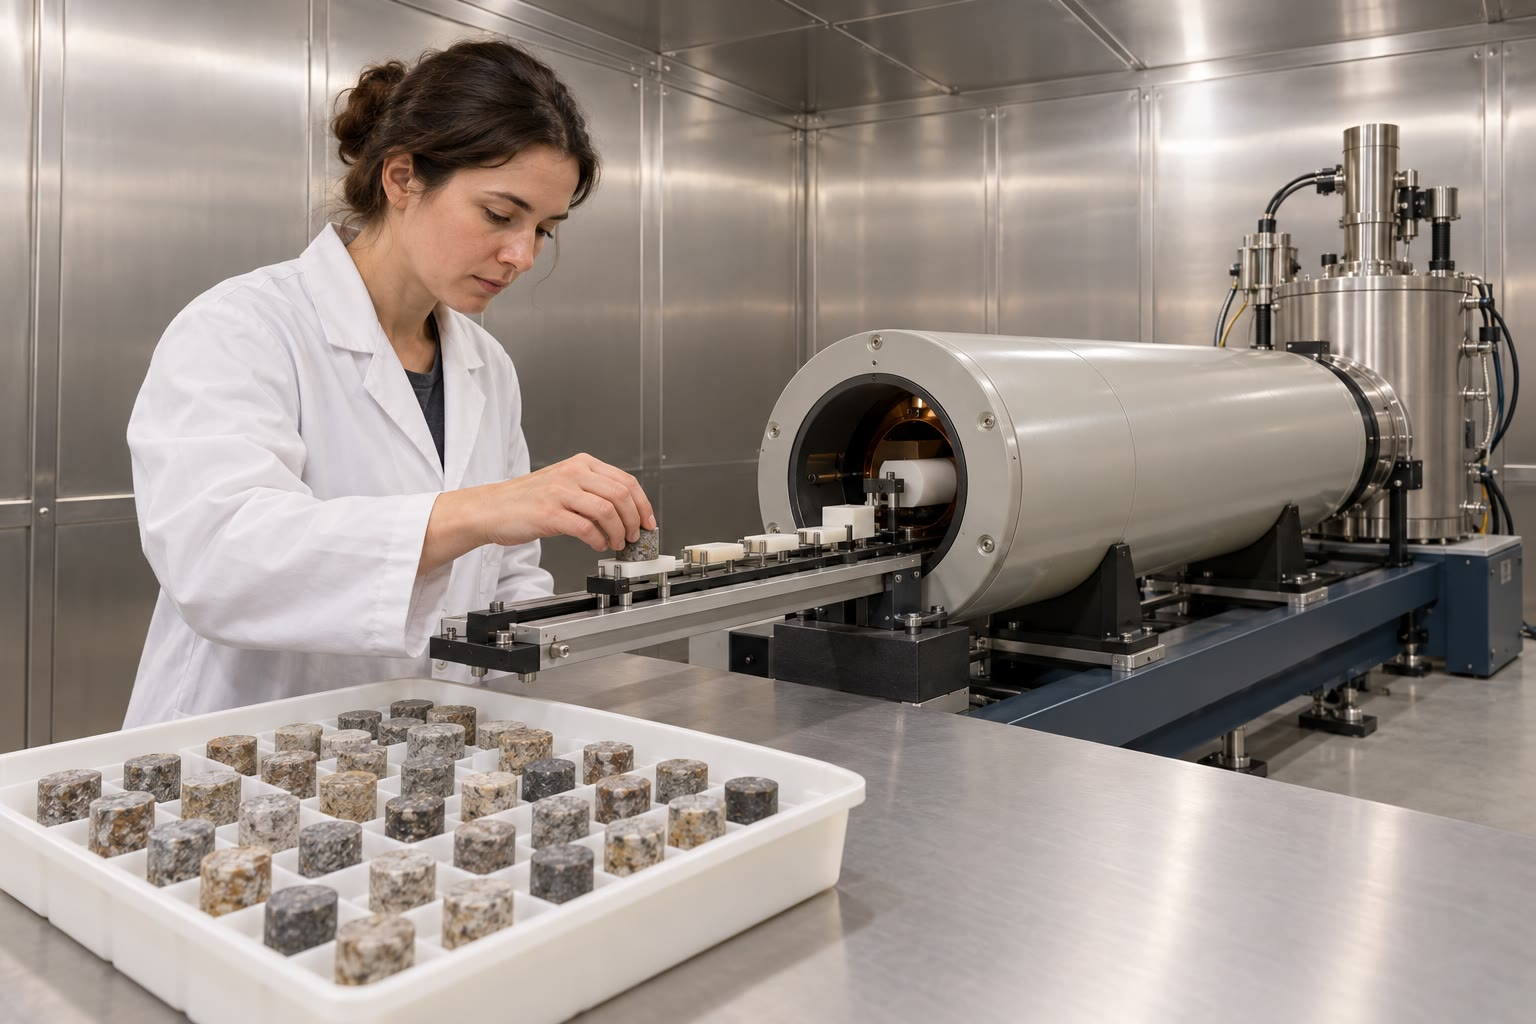
\includegraphics[width=\linewidth]{images/book5/ai/b3-palaeomag-lab.jpg}

{\scriptsize परिरक्षित कक्ष में एक चुंबकत्वमापी की नमूना-ट्रे पर नमूनों को लादना
(AI से बनाया गया चित्रण)।}
\end{minipage}
\end{inthelab}

\section{अभ्यास}

\begin{exercise}[$\star$]\label{exo:b3:palaeomagnetism:1}
\omterm{def:b3:palaeomagnetism:main-field}{भूकेंद्रीय अक्षीय द्विध्रुव} क्षेत्र में, अक्षांश
\ang{30}\,N पर \omterm{def:b3:palaeomagnetism:inclination}{चुंबकीय नति} परिकलित कीजिए, और वह अक्षांश ज्ञात कीजिए जिस स्थान पर \omterm{def:b3:palaeomagnetism:inclination}{चुंबकीय नति} \ang{-20} है।
\end{exercise}

\begin{exercise}[$\star$]\label{exo:b3:palaeomagnetism:2}
एक स्थान पर क्षेत्र के घटक $X = \qty{20000}{nT}$, $Y =
\qty{-2000}{nT}$ और $Z = \qty{40000}{nT}$ हैं। $H$, $F$, चुंबकीय क्रांति और
\omterm{def:b3:palaeomagnetism:inclination}{चुंबकीय नति} परिकलित कीजिए।
\end{exercise}

\begin{exercise}[$\star$]\label{exo:b3:palaeomagnetism:3}
2025 में, $g_1^0 = \qty{-29350}{nT}$। क्षेत्र को अक्षीय द्विध्रुव मानकर
भूमध्य रेखा और ध्रुवों पर क्षेत्र, तथा द्विध्रुव आघूर्ण परिकलित कीजिए।
($a = \qty{6371.2}{km}$, $\mu_0 = 4\pi\times\qty{e-7}{H.m^{-1}}$).
\end{exercise}

\begin{exercise}[$\star$]\label{exo:b3:palaeomagnetism:4}
निम्नलिखित प्रत्येक के लिए प्राप्त होने वाले अवशिष्ट चुंबकन का प्रकार, और वह कब क्षेत्र को अभिलिखित करता है, बताइए: (क) एक लावा प्रवाह का ठंडा होना;
(ख) एक शांत झील में गाद का जमना; (ग) एक बलुआ पत्थर, जिसकी
लौह ऑक्साइड परतें प्रारंभिक दफ़न के दौरान हेमेटाइट में बदल जाती हैं; (घ) एक बेसाल्ट जो
वर्तमान क्षेत्र में दस लाख वर्षों तक पड़ा रहता है।
\end{exercise}

\begin{exercise}[$\star\star$]\label{exo:b3:palaeomagnetism:5}
किसी स्थान के चार नमूने दिशाएँ $(D, I)$ देते हैं: $(\ang{12}, \ang{48})$,
$(\ang{22}, \ang{44})$, $(\ang{16}, \ang{57})$ और $(\ang{6}, \ang{53})$।
इनके एकांक सदिश, परिणामी लंबाई $R$, माध्य दिशा, $k$
और $\alpha_{95}$ परिकलित कीजिए।
\end{exercise}

\begin{exercise}[$\star\star$]\label{exo:b3:palaeomagnetism:6}
\ang{40.0}\,N, \ang{10.0}\,E पर स्थित एक स्थान की माध्य दिशा $D = \ang{20}$,
$I = \ang{50}$ है। इसका \omterm{def:b3:palaeomagnetism:vgp}{पुराअक्षांश} और \omterm{def:b3:palaeomagnetism:vgp}{आभासी भू-चुंबकीय ध्रुव} परिकलित कीजिए।
\end{exercise}

\begin{exercise}[$\star\star$]\label{exo:b3:palaeomagnetism:7}
IGRF 1900 में द्विध्रुव आघूर्ण \qty{8.32e22}{A.m^2} और
2025 में \qty{7.69e22}{A.m^2} देता है, और 2025 में $g_1^0$ के परिवर्तन की दर
\qty{+12.6}{nT/yr} देता है। (क) आघूर्ण का सापेक्षिक परिवर्तन प्रति शताब्दी
परिकलित कीजिए। (ख) यदि $g_1^0$ वही दर बनाए रखे, तो कितने वर्षों में वह शून्य तक पहुँचेगा?
यह पूर्वानुमान क्यों नहीं है?
\end{exercise}

\begin{exercise}[$\star\star$]\label{exo:b3:palaeomagnetism:8}
नमूने का शेष अवशिष्ट चुंबकन, \unit{mA/m} में (उत्तर, पूर्व, नीचे),
\qty{20}{\celsius} तक तापन के बाद $(32.2, 18.1, 38.2)$, \qty{300}{\celsius} के बाद $(25.8, 18.1, 24.6)$
और \qty{580}{\celsius} के बाद $(0.0, 0.0, 0.0)$ है; \omterm{def:b3:palaeomagnetism:zijderveld}{ज़ेडरवेल्ड आरेख}
हर जोड़ी के बीच सीधा है। 20 और \qty{300}{\celsius} के बीच हटाए गए घटक की दिशा और
तीव्रता, तथा \qty{300}{\celsius} से ऊपर हटाए गए घटक की, परिकलित कीजिए।
कौन-सा ChRM है, और
दूसरा क्या है?
\end{exercise}

\begin{exercise}[$\star\star$]\label{exo:b3:palaeomagnetism:9}
एक संरचना $I = \ang{-35}$ और $\alpha_{95} = \ang{5}$ देती है। इसका
\omterm{def:b3:palaeomagnetism:vgp}{पुराअक्षांश}, $I \pm \alpha_{95}$ द्वारा अनुमत पुराअक्षांशों का परास, और
उसके ध्रुव के विश्वास-दीर्घवृत्त के अर्ध-अक्ष $\mathrm dp$ और $\mathrm dm$
परिकलित कीजिए।
\end{exercise}

\begin{exercise}[$\star\star\star$]\label{exo:b3:palaeomagnetism:10}
 (क) \cref{thm:b3:palaeomagnetism:dipole} से वह अक्षांश, जहाँ
नति \ang{45} है, तथा ध्रुवों पर के क्षेत्र का
विषुवत रेखा पर के क्षेत्र से अनुपात ज्ञात कीजिए। (ख) दिखाइए कि $\mathrm dI/\mathrm d\lambda = 2/(1 + 3\sin^2\lambda)$,
और निष्कर्ष निकालिए कि नति की त्रुटि किस स्थान पर
\omterm{def:b3:palaeomagnetism:vgp}{पुराअक्षांश} में सबसे बड़ी त्रुटि देती है। (ग) कम नति से प्राप्त \omterm{def:b3:palaeomagnetism:vgp}{पुराअक्षांश}, अंशों में,
सबसे अधिक परिशुद्ध क्यों होते हैं?
\end{exercise}

\begin{exercise}[$\star\star\star$]\label{exo:b3:palaeomagnetism:11}
एक स्थल \ang{35.0}\,दक्षिण, \ang{150.0}\,पूर्व पर स्थित है, जो एक स्थिर प्लेट पर है, जिसका संदर्भ
ध्रुव, वहाँ नमूना लिए गए संरचना की आयु के लिए, \ang{70.0}\,उत्तर,
\ang{300.0}\,पूर्व पर है। (क) स्थल से ध्रुव तक की कोणीय दूरी $p$,
अपेक्षित नति और क्रांति, तथा अपेक्षित \omterm{def:b3:palaeomagnetism:vgp}{पुराअक्षांश} परिकलित कीजिए।
(ख) संरचना $D_o = \ang{30.0}$, $I_o = \ang{-60.0}$ देती है। घूर्णन $R$ और
ध्रुवाभिमुख विस्थापन $P$ परिकलित कीजिए, और बताइए कि वे क्या अर्थ रखते हैं।
\end{exercise}

\begin{exercise}[$\star\star\star$]\label{exo:b3:palaeomagnetism:12}
(क) \cref{prop:b3:palaeomagnetism:fisher} से दिखाइए कि किसी दिशा के
माध्य से $\theta$ के भीतर होने की प्रायिकता $(e^\kappa -
e^{\kappa\cos\theta})/(e^\kappa - e^{-\kappa})$ है। (ख) बड़े $\kappa$ और
छोटे $\theta$ के लिए दिखाइए कि यह लगभग $1 - e^{-\kappa\theta^2/2}$ है, और निष्कर्ष निकालिए
कि दिशाओं का \qty{63}{\percent} भाग $\theta_{63} \approx
\ang{81}/\sqrt\kappa$ के भीतर है। (ग) $\theta_{63}$ परिकलित कीजिए, जहाँ $\kappa = 50$ है,
और सटीक सूत्र से \qty{63}{\percent} की जाँच कीजिए।
\end{exercise}

\section{समस्या: केस्टा के लाल संस्तर}

\begin{problem}[{सप्ताहांत समस्या --- एक विस्थापित टेरेन की तीन संरचनाएँ,
उनकी दिशाएँ, ध्रुव और घूर्णन, तथा सबसे तरुण की आयु}]
\label{pb:b3:palaeomagnetism:1}
% values: calc/ch04.py; palaeomag_stats.py, magnetostratigraphy.py; GPTS: iodp:gpts2004
केस्टा एक काल्पनिक टेरेन है, जो अब \ang{47.0}\,उत्तर, \ang{15.0}\,पूर्व पर है, और एक काल्पनिक स्थिर महाद्वीप के
किनारे पर है। इसमें तीन लाल संस्तर संरचनाएँ दिखती हैं: A,
\qty{60}{Ma}; B, \qty{30}{Ma}; C, लगभग 3.7 से \qty{2.4}{Ma} तक। प्रत्येक से
कई स्थलों पर नमूने लिए गए, और हर नमूने का तापीय विचुंबकन किया गया। ChRM
का वाहक हीमेटाइट है, और संरचनाएँ क्षैतिज हैं।

\medskip\noindent\textbf{भाग I --- माध्य दिशाएँ।} संरचना A के छह स्थल
$(D, I)$ देते हैं: $(\ang{50}, \ang{37})$, $(\ang{28}, \ang{37})$,
$(\ang{21}, \ang{42})$, $(\ang{24}, \ang{27})$, $(\ang{37}, \ang{39})$,
$(\ang{46}, \ang{38})$।
\begin{enumerate}
  \item लाल संस्तर में हीमेटाइट द्वारा वाहित ChRM संस्तर से तरुण क्यों हो सकता है?
        किस बात से दिखेगा कि वह बहुत तरुण नहीं है?
  \item पहली दिशा का इकाई सदिश परिकलित कीजिए।
  \item छह इकाई सदिशों का योग $(3.8943, 2.6500, 3.5717)$ है। $R$ और
        संरचना A की माध्य दिशा परिकलित कीजिए।
  \item संरचना A के लिए $k$ और $\alpha_{95}$ परिकलित कीजिए।
  \item संरचना B देती है, 7 स्थलों से, $D = \ang{23.9}$, $I = \ang{51.5}$ और
        $R = 6.8979$; संरचना C, 8 स्थलों से, $D = \ang{3.4}$, $I =
        \ang{63.7}$ और $R = 7.8707$। प्रत्येक के लिए $k$ और $\alpha_{95}$ परिकलित कीजिए।
  \item कौन-सी संरचना सबसे अच्छी तरह समूहित है? कौन-सा माध्य सबसे अच्छी तरह परिभाषित है?
\end{enumerate}

\medskip\noindent\textbf{भाग II --- पुराअक्षांश और ध्रुव।}
\begin{enumerate}[resume]
  \item A, B और C के \omterm{def:b3:palaeomagnetism:vgp}{पुराअक्षांश} परिकलित कीजिए।
  \item संरचना A के लिए पुरा-सहअक्षांश $p$ और उसके
        \omterm{def:b3:palaeomagnetism:vgp}{आभासी भू-चुंबकीय ध्रुव} का अक्षांश परिकलित कीजिए।
  \item उस ध्रुव का देशांतर परिकलित कीजिए, और जाँचिए कि
        \cref{thm:b3:palaeomagnetism:pole} की कौन-सी स्थिति लागू होती है।
  \item A के ध्रुव के लिए $\mathrm dp$ और $\mathrm dm$ परिकलित कीजिए।
  \item B और C के ध्रुव \ang{66.5}\,उत्तर, \ang{135.6}\,पूर्व और
        \ang{87.1}\,उत्तर, \ang{139.1}\,पूर्व पर हैं। तीनों ध्रुवों के पथ का
        आयु के साथ वर्णन कीजिए।
\end{enumerate}

\medskip\noindent\textbf{भाग III --- संरचना C की आयु।} संरचना C में,
आधार से नमूने \qty{4.2}{m} तक उत्क्रमित हैं, \qty{14.8}{m} तक सामान्य,
\qty{19.7}{m} तक उत्क्रमित, \qty{24.6}{m} तक सामान्य, \qty{29.2}{m} तक उत्क्रमित
और \qty{54.0}{m} तक सामान्य, फिर शीर्ष तक उत्क्रमित, जो
\qty{64.0}{m} पर है। \qty{22}{m} पर एक राख संस्तर की आयु लगभग \qty{3.2}{Ma} निर्धारित हुई है।
क्रॉन C2An के सामान्य उपक्रॉन 3.596--3.330, 3.207--3.116 और
3.032--\qty{2.581}{Ma} फैले हैं।
\begin{enumerate}[resume]
  \item राख संस्तर का उपयोग करते हुए ध्रुवता क्षेत्रों का समय-पैमाने से मिलान कीजिए।
  \item पहली और तीसरी उत्क्रमण सीमा के बीच, तथा
        चौथी और छठी सीमा के बीच की संचयन दर परिकलित कीजिए।
  \item खंड के आधार और शीर्ष की आयु का अनुमान लगाइए।
  \item दर सैकड़ों हज़ार वर्षों पर माध्य क्यों है, और
        कौन-सी बात इसे बदल सकती है?
\end{enumerate}

\medskip\noindent\textbf{भाग IV --- स्थिर महाद्वीप के सापेक्ष, और विस्थापन।} स्थिर महाद्वीप के
संदर्भ ध्रुव \ang{78.0}\,उत्तर, \ang{190.0}\,पूर्व
($A_{95} = \ang{3.0}$) \qty{60}{Ma} पर; \ang{83.5}\,उत्तर, \ang{175.0}\,पूर्व
($\ang{2.5}$) \qty{30}{Ma} पर; और \ang{87.5}\,उत्तर, \ang{150.0}\,पूर्व ($\ang{2.0}$)
\qty{4}{Ma} पर।
\begin{enumerate}[resume]
  \item केस्टा से \qty{60}{Ma} संदर्भ
        ध्रुव तक की कोणीय दूरी, तथा अपेक्षित नति और \omterm{def:b3:palaeomagnetism:vgp}{पुराअक्षांश} परिकलित कीजिए।
  \item \qty{60}{Ma} पर अपेक्षित क्रांति परिकलित कीजिए।
  \item 30 और \qty{4}{Ma} पर अपेक्षित दिशाएँ $(\ang{2.9},
        \ang{60.0})$ और $(\ang{2.5}, \ang{63.6})$। A, B और C का ध्रुवाभिमुख
        विस्थापन $P$ परिकलित कीजिए।
  \item A, B और C का घूर्णन $R$ परिकलित कीजिए।
  \item A के लिए त्रुटियाँ $\Delta D_o$ और $\Delta D_x$ तथा
        उसके घूर्णन की त्रुटि परिकलित कीजिए।
  \item B और C के लिए $R$ की त्रुटियाँ \ang{13.8} और \ang{17.9} हैं। कौन-से
        घूर्णन 95 प्रतिशत स्तर पर सार्थक हैं?
  \item स्थिर महाद्वीप के सापेक्ष केस्टा का इतिहास बताइए।
  \item केस्टा का संरचना A से लेकर उत्तर की ओर विस्थापन, घूर्णन अक्ष के सापेक्ष,
        डिग्री और किलोमीटर, दोनों में, परिकलित कीजिए
        (\qty{111.19}{km} प्रति डिग्री)।
  \item $I \pm \alpha_{95}$ द्वारा अनुमत \omterm{def:b3:palaeomagnetism:vgp}{पुराअक्षांश} संरचना A के लिए
        परिकलित कीजिए, और उस अंतराल की चौड़ाई के आधे को
        1.96 से भाग देकर प्राप्त मान को एक मानक विचलन मानिए। संरचना A से लेकर
        केस्टा का उत्तर की ओर विस्थापन, किलोमीटर में, उसके मानक विचलन सहित दीजिए।
\end{enumerate}
\end{problem}
